\documentclass[12pt,a4paper]{book}
\usepackage[latin1]{inputenc}
\usepackage{amsmath}
\usepackage{amsfonts}
\usepackage{amssymb}
\usepackage{graphicx}
\usepackage{cleveref}
\usepackage{tikz}
\usepackage{bm}
\usepackage{enumerate}
\usetikzlibrary{bayesnet}
\usepackage[left=2.00cm, right=2.00cm, top=2.00cm, bottom=2.00cm]{geometry}
\author{Demetri Pananos}
\title{Bayesian Pharmacokinetic Models}
\usepackage{fancyhdr}
\pagestyle{fancy}
\fancyhf{}
\lhead{Baysian Pharmacokinetic Models}
\rhead{Pananos 2019}
\rfoot{Page \thepage}
\begin{document}
\maketitle

\section{Derivation of the Differential Equation For Concentration}

A dose of size $ D $ is orally administered to a patient. The rate of drug absorption from the gut $ G $ into the blood plasma $ C $ is proportional to the concentration of drug in the gut.  The proportionality constant in this case is $ k_a $ (the $ a $ stands for ``absorption'').

The drug is eliminated from the blood plasma at a rate proportional to the concentration of drug currently in the blood plasma.  The proportionality constant in this case is $ k_e $ (the $ e $ stands for ``excretion'').
%
\begin{figure}[h!]
	\centering
	\tikzstyle{int}=[draw, fill=white, minimum size=2em]
	\tikzstyle{init} = [pin edge={to-,thin,black}]
	\begin{tikzpicture}[node distance=2.5cm,auto,>=latex']
	\node [int] (a) {$G$};
	\node (b) [left of=a,node distance=2cm, coordinate] {a};
	\node [int] (c) [right of=a] {$C$};
	\node [coordinate] (end) [right of=c, node distance=2cm]{};
	\path[->] (a) edge node {$k_a$} (c);
	\draw[->] (c) edge node {$k$} (end) ;
	\end{tikzpicture}
	\caption[Pharmacokinetic compartmental diagram]{A compartmental diagram for a one compartment pharmacokinetic model.  Arrows indicate the direction of flux.  Flux is proportional to the concentration in each compartment, with proportionality constant indicated over the arrows.}
	\label{compartmental_diagram}
\end{figure}

I can write this system as a differential equation, namely

\begin{align}\label{pk_odes}
	\dfrac{dG}{dt} &= -k_aG(t) \quad G(0) = D/V\\
	\dfrac{dC}{dt} &= k_aG(t) - k_e C(t) \quad C(0) = 0 \>.
\end{align}

\noindent Here $ V $ is the volume of blood plasma in the body and is assumed to be constant over time. The differential equation for $G$ is uncoupled from the differential equation for $C$, so I can solve for $G$ and substitute this solution into the differential equation for $C$.  This results in the following differential equation, which describes the concentration of the drug in the blood plasma over time

\begin{equation}
	\dfrac{dC}{dt} = \dfrac{D}{V}k_a\exp(-k_at) - k_eC(t) \quad C(0) = 0 \>.
\end{equation}

\noindent Through the relation $ V=Clk_e $, where $ Cl $ is the rate of total body drug clearance, a form more amenable to analysis is obtained.  Thus, the dynamics of concentration hereforth are modeled using

\begin{equation}
	\dfrac{dC}{dt} = \dfrac{D}{Cl}k_ek_a\exp(-k_at) - k_eC(t) \quad C(0) = 0
\end{equation}

\noindent which has solution

\begin{equation}
C(t) = \dfrac{D}{Cl} \dfrac{k_ak_e}{k_a - k_e}\Big( \exp({-k_et}) - \exp({-k_at}) \Big)
\end{equation}

\noindent The benefit of this parmaeterization is that the area under the curve $ T_\infty $ is given by $ D/Cl $.

\section{Non-Dimensionalization Gives Insight For Prior Selection}

Non-dimensionalization will become useful as I begin to select priors for the various hyperparameters of our eventual Bayesian model.  To begin, I list all the dimensions of the parameters.  In the table below $ M $ indicates units in mass, $ V $ indicates units in volume,  and $ T $ indicate units in time.

\begin{center}
	\begin{tabular}{ |c|c| } 
		\hline
		Parameter & Units  \\
		\hline
		$ D $ &  $ M $\\
		$Cl$  & $ VT^{-1} $\\
		$ k_a $ & $ T^{-1} $\\
		$ k_e $  & $ T^{-1} $\\
		\hline
		\hline
	\end{tabular}
\end{center}

Let $ y $ and $ \tau $ be non-dimensional concentration and time variables such that 

\begin{align}
 C = \dfrac{Dke}{Cl}y \\
 t = \dfrac{\tau}{k_a}
\end{align}

\noindent The non-dimensionalization results in

\begin{align}
\dfrac{dy}{d\tau} &= \dfrac{dt}{d\tau}\dfrac{Cl}{Dk_e} \left(\dfrac{dC}{dt}\right)\\
 &=\dfrac{1}{k_a}\dfrac{Cl}{Dk_e}\Big(\dfrac{D}{Cl}k_ek_a\exp(-k_at) - k_eC(t)\Big)\\
&= \exp(-\tau) - \alpha y(\tau)
\end{align}

\noindent  The non-dimensionalization constant is $ \alpha=k_e/k_a $.



\section{Bayesian Hierarchical Model With No Covariates}

Shown below is a Bayes' net describing the hierarchical structure.  In what follows, I further explain and rationalize the model structure.


\begin{figure}[h!]
	\centering
	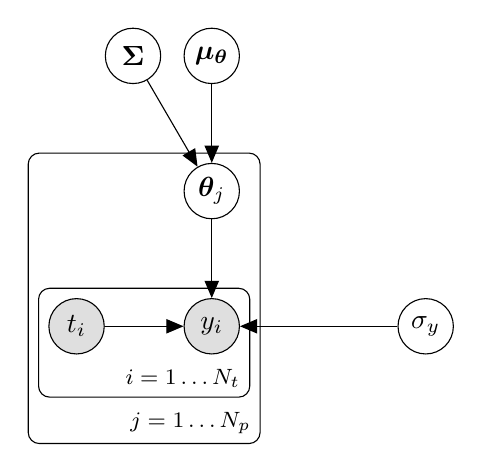
\begin{tikzpicture}
	
	\node[obs](y){$y_i$};
	\node[latent, above = of y](theta){$\bm{\theta}_j$};
	\node[latent, above = of theta](mu_theta){$\bm{\mu_{\theta}}$};
	\node[latent, above = of theta, xshift = -1 cm](Sig){$\bm{\Sigma}$};
	\node[latent, right = of y, xshift = 1 cm](sig){$\sigma_y$};
	\node[obs, left = of y](t){$t_i$};
	
	
	\edge{theta}{y};
	\edge{Sig}{theta};
	\edge{mu_theta}{theta};
	\edge{sig}{y};
	\edge{t}{y};
	
	\plate{t_y_pairs}{(t)(y)}{$i=1\dots N_t$};
	\plate{patient_level}{(theta)(t_y_pairs)}{$j = 1\dots N_p$};
	\end{tikzpicture}
	\caption{Bayes net for first pharmacokinetic model.  Parameters here are shown to be modelled jointly but are assumed independent.}
	\label{model_2}
\end{figure}

In the Bayes' net above, I have concatenated the parameters $ Cl $, $ k_e $, and $ k_a $ into a single random vector $ \bm{\theta} $ for economy of thought.  The parameters will be independent in the joint distribution.  The population level means for these parameters is $\bm{\mu_{\theta}}$.  Since all parameters are taken to be positive, I model these parameters on the log scale and then later exponentiate. The priors for $ \mu_{Cl} $ and $ \mu_{k_e} $ are

\begin{align}
	\log(\mu_{Cl}) &\sim \mathcal{N}(\cdot, \cdot)\\
	\log(\mu_{k_e}) &\sim \mathcal{N}(\cdot, \cdot)
\end{align}

The exception is for $ \log(k_a) $.  This model is known to display ``Flip-Flop` kinetics; a different dynamic regime occurs when the non-dimensionalization parameter crosses 1.  The details of absorption for most drugs \textit{should} be well know (for instance, an estimate for time max concentration).  Using this information should give insight into if $ \alpha<1 $ or $ \alpha>1 $.  In this case, I assume $\alpha<1$ implying $ k_e<k_a $.  The non-dimensionalization thus allows for the following parameterization for $ \log(k_a) $

\begin{align}
\alpha &\sim \operatorname{Beta}(\cdot, \cdot)\\
\log(k_a) &= \log(k_e) - \log(\alpha) > \log(k_e)
\end{align}

\noindent Since $ 0<\alpha<1 $, then $ -\log(\alpha)>0 $, and since the logarithm is monotonically increasing, the inequality $ k_e < k_a $ is preserved through this parameterization.  Furthermore, pharmacokinetic expertise can be leveraged to put an appropriate prior on $ \alpha $.

In the next stage of the hierarchy, the pharmacokinetic parameters are drawn a lognormal density.  The conditional density at this stage is coded using a non-central parameterization to help the HMC sampler explore the posterior more easily.  To reflect that parameterization, I've written the conditional density in the same manner, namely  

\begin{align}
	z^{Cl}_j &\sim \mathcal{N}(0,1)\\
	\sigma_{Cl} &\sim \operatorname{Cauchy}(0,1)\\
	Cl_j &= \exp\Big(\log(\mu_{Cl}) + z^{Cl}_j\sigma_{Cl}\Big) \\ \nonumber\\
	z^{k_e}_j &\sim \mathcal{N}(0,1)\\
	\sigma_{k_e} &\sim \operatorname{Cauchy}(0,1)\\
	k_{e_j} &= \exp\Big(\log(\mu_{k_e}) + z^{k_e}_j\sigma_{k_e}\Big) \\ \nonumber \\
	z^{k_a}_j &\sim \mathcal{N}(0,1)\\
	\sigma_{k_a} &\sim \operatorname{Cauchy}(0,1)\\
	k_{a_j} &= \exp\Big(\log(\mu_{k_a}) + z^{k_a}_j\sigma_{k_a}\Big)
\end{align}
 
 \noindent Here, I have put halff-cauchy priors on the $ \sigma $.  These ought to be changed to something more realistic, but serve as good-enough in scenarios where practitioners are uncertain about noise estimates.  Once the pharmacokinetic parameters are drawn, predictions are made by evaluating $C(t)$ with the drawn parameters.  The likelihood is then
 
  \begin{equation}
 \log(y_{i,j}) \vert t, Cl_{j}, k_{a_j}, k_{e_j} \sim \mathcal{N}(\log(C(t)), \sigma^2_y)
 \end{equation}
 
 Here, a half Cauchy prior can be placed on $\sigma^2_y$ for convenience.  However, pharmacokinetic expertise says that the machinery used to detect these drug levels is guaranteed to be within 10\% of the true value (according to the manufacturer). This could be used to justify a more precise prior.
 
\section{Extensions}

The model proposed above can be extended easily to perform regression by specifying a prior over regression parameters 

\begin{align}
	\bm{\beta}_{Cl} &\sim p(\beta_{Cl})\\
	\log(\mu_{Cl}) &= \mathbf{X}\bm{\beta}_{Cl}
\end{align}

\noindent The prior in this instance could also serve to regularize coefficient estimates so as to select only predictive variables (think Bayesian lasso).  My only worry here is that the effects are likely already very close to 0, which may make selection difficult.  Anyway, no way to now know, we could always do yet another simulation.

\section{Time Delay Effects}

Time delays can be modelled as follows.  Assume patient $ j $'s first non-zero measurement is observed at $ \tau_j $.  The concentration at this time is $ C_j(\tau_j - \delta_j) $, where $ \delta_j $ is patient $ j $'s time delay.

Assume each patient has their own time delay which comes from some population delay distribution.  Thus, the model structure for the delay is

 \begin{align}
	\mu_{\delta} &\sim p(\mu_{\delta})\\
	\kappa_{\delta} &\sim p(\kappa_{\delta})\\
	\delta_j &\sim \operatorname{Beta}\Big(\mu_{\delta}\kappa_{\delta}, (1-\mu_{\delta})\kappa_{\delta}\Big)\\
	t_{j,actual} &= t_{j,obs} - \tau_j\delta_j
 \end{align}
 
 \noindent Here, $ t_{j, actual} $ is the actual time after absorption of the drug for the $ j^{th} $ patient, and  $p$ is an appropriate prior for $ \mu_{\delta} $ and $ \kappa_{\delta} $.


\section{Model Evaluation}

The goal of these models is to predict concentrations for out of sample patients.  I could compare RMSE between models, or I could evaluate the some information criterion.  The problem with these approaches is that they utilize \textit{observations} rather than true concentrations to evaluate how well the model predicts on unseen data.  After all, observations are noisy, and we aren't so interested in predicting observed concentrations so much as we are interested in predicting actual concentrations.

Sampling pharmacokinetic parameters from the posterior allows us to in essence sample functions since $ \hat{C}(t) $ is determined by the parameters. In a simulation study, we can compare the $ \hat{C}(t) $ to $ C(t) $ directly by computing the $ \ell_2 $ norm

\begin{equation}
 \mbox{Error}^2 = \left<C(t), \hat{C}(t)\right> = \int_{0}^\infty \lvert  C(t) - \hat{C}(t)\rvert^2 \, dt
\end{equation}

\noindent Since $ C(t) $ is comprised of elementary functions, the evaluation of this integral can be done exactly using computer algebra, and made a function of the parameters for $ C(t) $ and $ \hat{C}(t) $.

Other pharmacokinetic phenomena can be evaluated similarly.  The time to max concentration is 


\begin{equation}
t_{max} = \dfrac{\log(k_a) - \log(k_e)}{k_a - k_e}
\end{equation}

\noindent and so bias and RMSE for this quantity, as well as the max achieved  concentration, $ C(t_{max}) $, and area under the curve, $ T_\infty $,  can be evaluated easily.


\section{What Have Other People Done?  Why Do This?}


\subsection{Calling the Kettle Black; I Am The Dogmatic One}
I have believed from the start that ``Bayes will save us'' because 

\begin{enumerate}[i)]
 \item Small samples per patient
 \item Prior knowledge
 \item Conditioning on new information
\end{enumerate}

I think it is worth examining these presuppositions in a simulation study.  How well do our models perform when we have small samples (as small and as sparse as the personalized medicine clinic has)?  How well do weakly informative priors do in terms of out of sample prediction error, but also in terms of bias and RMSE for parameter estimation? When is it worth while to have informative priors? Is it better to collect a bunch of possibly informative covariates, or are we better just observing patients for a little while and letting our model learn from that?

\subsection{NONMEM Is Dominant}

Nearly all the pharmacokinetic papers I've read have used NONMEM to model pharmacokinetics.  That is well and great, but if free open source tools (like Stan, like PyMC3) are not being used, I think it is important to as ``why not?''.  Worst case scenario, these tools do worse than the NONMEM, but that in and of itself would be a useful result not only for the PK community but also for open source.  Best case scenario the open source tools do better, which I'm sure the creators of NONMEM would love to know.  Most probably case is that they do equally well, in which case everyone wins.

\subsection{Principled Evaluation of Models}
 
 A lot of the PK models I've seen often use questionable methods for evaluation (e.g. multiple hypothesis tests looking for $ p<0.05 $). It would be nice to introduce a principled way to evaluate these sorts of models for fit.  I'm not quite sure how I would do that just yet.


\end{document}